


\begin{frame}{Exploratory Modeling \sof{1}{2}}

\vspace{1em}
\justifying
After resigning from my research position at the DFKI and joining 
\lnk{https://mci.fernuni-hagen.de}{Prof. Peters} at the University of Hagen 
{\bf I refocused my work} away from robotic engineering towards more fundamental 
research aimed at understanding the {\bf processing of information in 
neurobiological systems} -- a topic I pursued already during my spare time at 
the DFKI. 

\vspace{1.5em}
As a basis for this new direction of research we investigated how the 
{\bf understanding of complex systems} can be improved {\bf by methods of 
exploratory modeling and simulation}.

%\vspace{-1em}

\begin{columns}[t]
\begin{column}{0.36\textwidth}
\begin{figure}
{
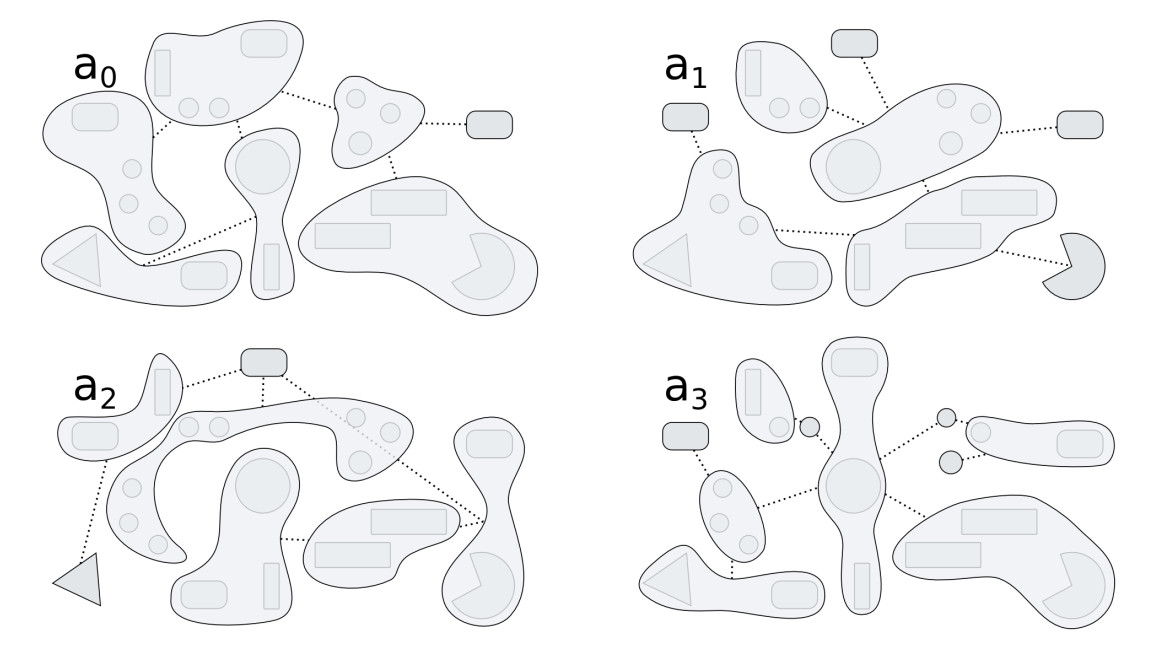
\includegraphics[width=\linewidth]{exploratory_modeling/aspects.jpg}
}

\vspace{-1.0em}
\caption{\justifying\scriptsize The constituents of a complex system may change
when analyzed regarding different aspects~\cite{Kerdels2012}.}
\end{figure}
\end{column}
\begin{column}{0.2\textwidth}

\vspace{1.5em}
\begin{figure}
{
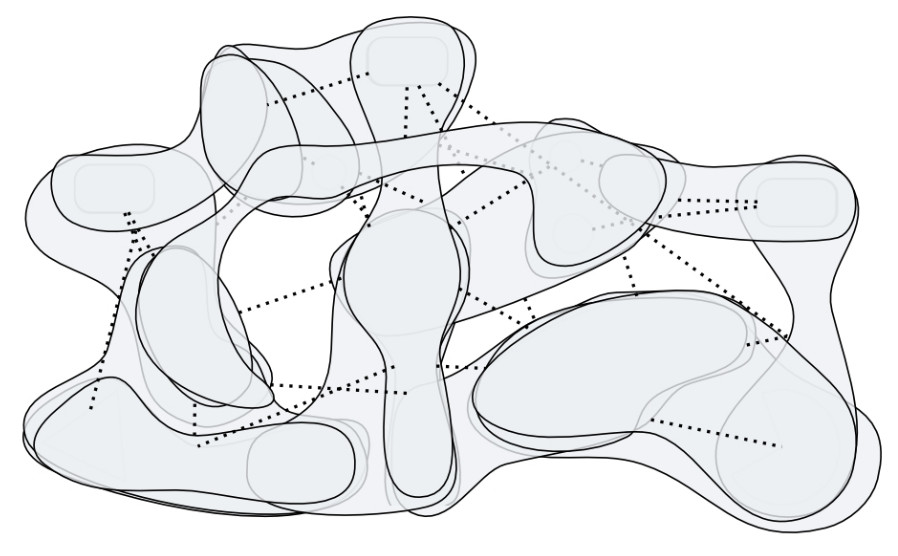
\includegraphics[width=\linewidth]{exploratory_modeling/merged.jpg}
}

\vspace{-0.5em}
\caption{\scriptsize Resulting constituents can ``conceptually overlap'' when
they are merged into a single model~\cite{Kerdels2012}.}
\end{figure}
\end{column}
\begin{column}{0.34\textwidth}
\begin{figure}
{
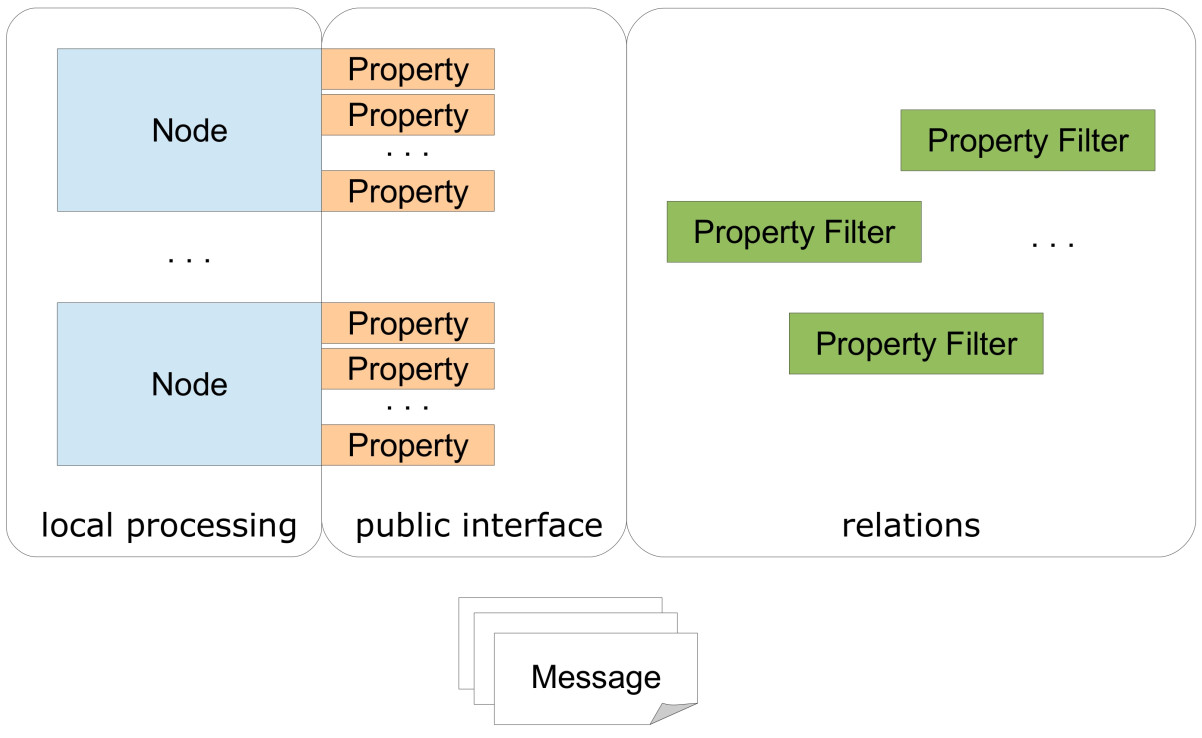
\includegraphics[width=\linewidth]{exploratory_modeling/genmodel.jpg}
}

\vspace{-0.75em}
\caption{\scriptsize Components of the proposed generalized model~\cite{Kerdels2012}.}
\end{figure}
\end{column}
\end{columns}	


\begin{center}
\rule{2cm}{0.4pt}\\[0.5em]
\end{center}

\fc{Kerdels2012}{publications/2012-01/2012-01}


\end{frame}


\begin{frame}{Exploratory Modelling \sof{2}{2}}

%\vspace{1em}
\justifying
In~\cite{Kerdels2012} we {\bf identify key aspects} that make modeling complex 
systems difficult:

\begin{itemize}
	\item The relations between the constituents of a complex system can vary
    over time in non-trivial ways and thus cannot be specified in advance.
    \item Mutual influences between constituents of a complex system are not 
    only represented by higher-level categories as in complicated systems but 
    are also indicated by shared, lower-level categories.
    \item If a complex system is analyzed with respect to different aspects, the
    resulting constituents for each aspect can ``conceptually overlap'' when 
    they are merged into a single model of the system.
\end{itemize}

\vspace{1em}
Using a computational modeling perspective we reduced the problem space further
to a single problem that we call the {\bf addressing problem}.

\vspace{1em}
As a solution to the addressing problem we propose a {\bf generalized 
computational model} that is tailored to the specific needs of modeling and 
simulating complex systems~\cite{Kerdels2012,Kerdels2013a}.

%\vspace{-0.5em}

\begin{center}
\rule{2cm}{0.4pt}\\[0.5em]
\end{center}

\fc{Kerdels2013a}{publications/2013-02/2013-02}

\end{frame}


